\begin{figure}[htb]
	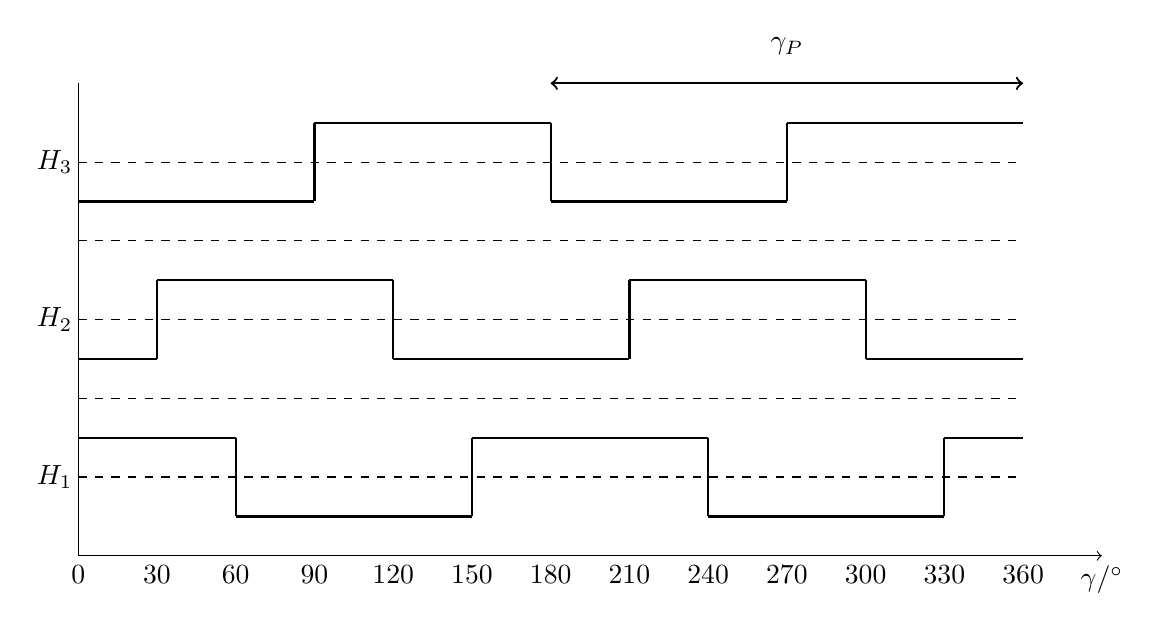
\begin{tikzpicture}
	
	% horizontal axis
	\draw[->] (0,0) -- (13,0) node[anchor=north] {$\gamma/^{\circ}$};
	\draw[dashed] (0, 1) -- (12,1);
	\draw[dashed] (0, 2) -- (12,2);
	\draw[dashed] (0, 3) -- (12,3);
	\draw[dashed] (0, 4) -- (12,4);
	\draw[dashed] (0, 5) -- (12,5);

	% vertical axis
	\draw (0,0) -- (0,6) node[anchor=east] {};

	% labels
	\draw	
	(0,0) node[anchor=north] {0}
	(1,0) node[anchor=north] {30}
	(2,0) node[anchor=north] {60}
	(3,0) node[anchor=north] {90}	
	(4,0) node[anchor=north] {120}
	(5,0) node[anchor=north] {150}
	(6,0) node[anchor=north] {180}
	(7,0) node[anchor=north] {210}
	(8,0) node[anchor=north] {240}
	(9,0) node[anchor=north] {270}
	(10,0) node[anchor=north] {300}
	(11,0) node[anchor=north] {330}
	(12,0) node[anchor=north] {360};	
	
	\draw (-0.3, 5) node{{$H_3$}};
	\draw (-0.3, 3) node{{$H_2$}};
	\draw (-0.3, 1) node{{$H_1$}};

	%draw H3
	\draw [thick] 
	(0, 4.5) --  (3, 4.5)
	(3, 4.5) --  (3, 5.5)
	(3, 5.5) --  (6, 5.5)
	(6, 5.5) --  (6, 4.5)
	(6, 4.5) --  (9, 4.5)
	(9, 4.5) --  (9, 5.5)
	(9, 5.5) -- (12, 5.5);
	
	%draw H2
	\draw [thick] 
	(0, 2.5)  --  (1, 2.5)
	(1, 2.5)  --  (1, 3.5)
	(1, 3.5)  --  (4, 3.5)
	(4, 3.5)  --  (4, 2.5)
	(4, 2.5)  --  (7, 2.5)
	(7, 2.5)  --  (7, 3.5)
	(7, 3.5)  -- (10, 3.5)
	(10, 3.5) -- (10, 2.5)
	(10, 2.5) -- (12, 2.5);	
	
	%draw H1
	\draw [thick] 
	(0, 1.5)  --  (2, 1.5)
	(2, 1.5)  --  (2, 0.5)
	(2, 0.5)  --  (5, 0.5)
	(5, 0.5)  --  (5, 1.5)
	(5, 1.5)  --  (8, 1.5)
	(8, 1.5)  --  (8, 0.5)
	(8, 0.5)  -- (11, 0.5)
	(11, 0.5) -- (11, 1.5)
	(11, 1.5) -- (12, 1.5);

	%draw gamme_P
	\draw [thick, <-]
	(6, 6) -- (9, 6);
	\draw [thick, ->]
	(9, 6) -- (12, 6);
	\draw 
	(9, 6.7) node[anchor=north] {$\gamma_P$};
	
	
	\end{tikzpicture}
	\caption{Signale der Hallsensoren bei $Z_P = 2$}
	\label{dia:aufg3a_hall}
\end{figure}
